\documentclass[12pt,letterpaper]{article}
\usepackage{amsmath} % just math
\usepackage{amssymb} % allow blackboard bold (aka N,R,Q sets)
\usepackage{ulem}
\usepackage{graphicx}
\usepackage{float}
\linespread{1.6}  % double spaces lines
\usepackage[left=1in,top=1in,right=1in,bottom=1in,nohead]{geometry}
\usepackage{caption}
\usepackage{subcaption}
\usepackage{floatrow}
\usepackage{blindtext}


\begin{document}
\setcounter{subsection}{2} 
\begin{flushright}
\end{flushright}
\begin{flushleft}
\textbf{Eric Zounes, Ian Fridge} \\
\today \\ 
CS434: Assignment 3
\end{flushleft}
\section[1]{Implementation Assignment} 
\begin{enumerate} 
	\item[1.] Implementing K-Means 	
	\begin{enumerate} 
		\item Run your kmeans algorithm with $k = 3$. To verify that your algorithmn actually converges, please plot the objective of the Kmeans algorithm (SSE) as a function of the iterations. From one run to another run, this curve may look different. Just present the results of a typical run. \\
		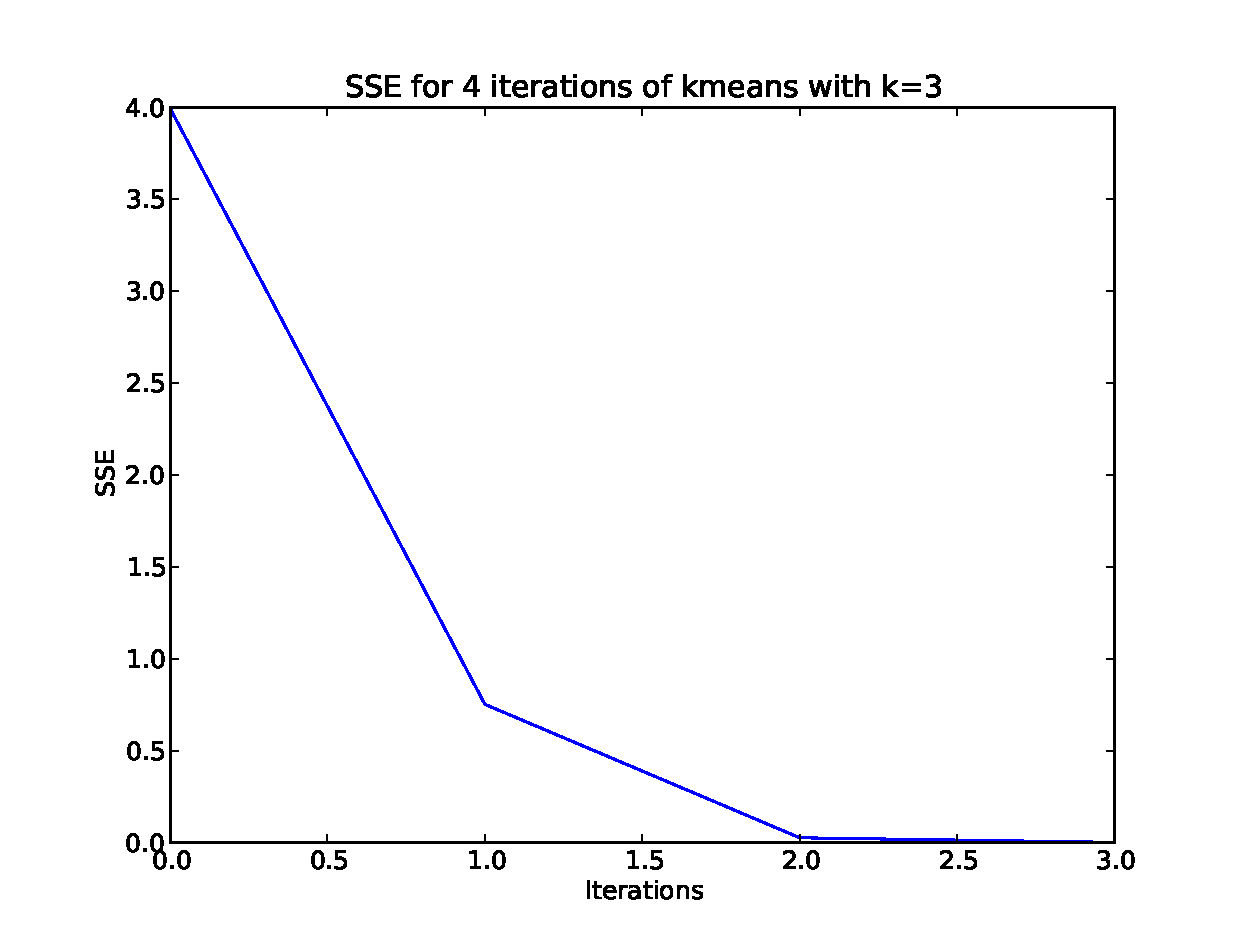
\includegraphics[width=6in]{SSEk3.eps} \\[15mm]
		\item Plot the scatter plot of the given data, and inspect the scatter plot visually. How many clusters do you see in this data? \\
		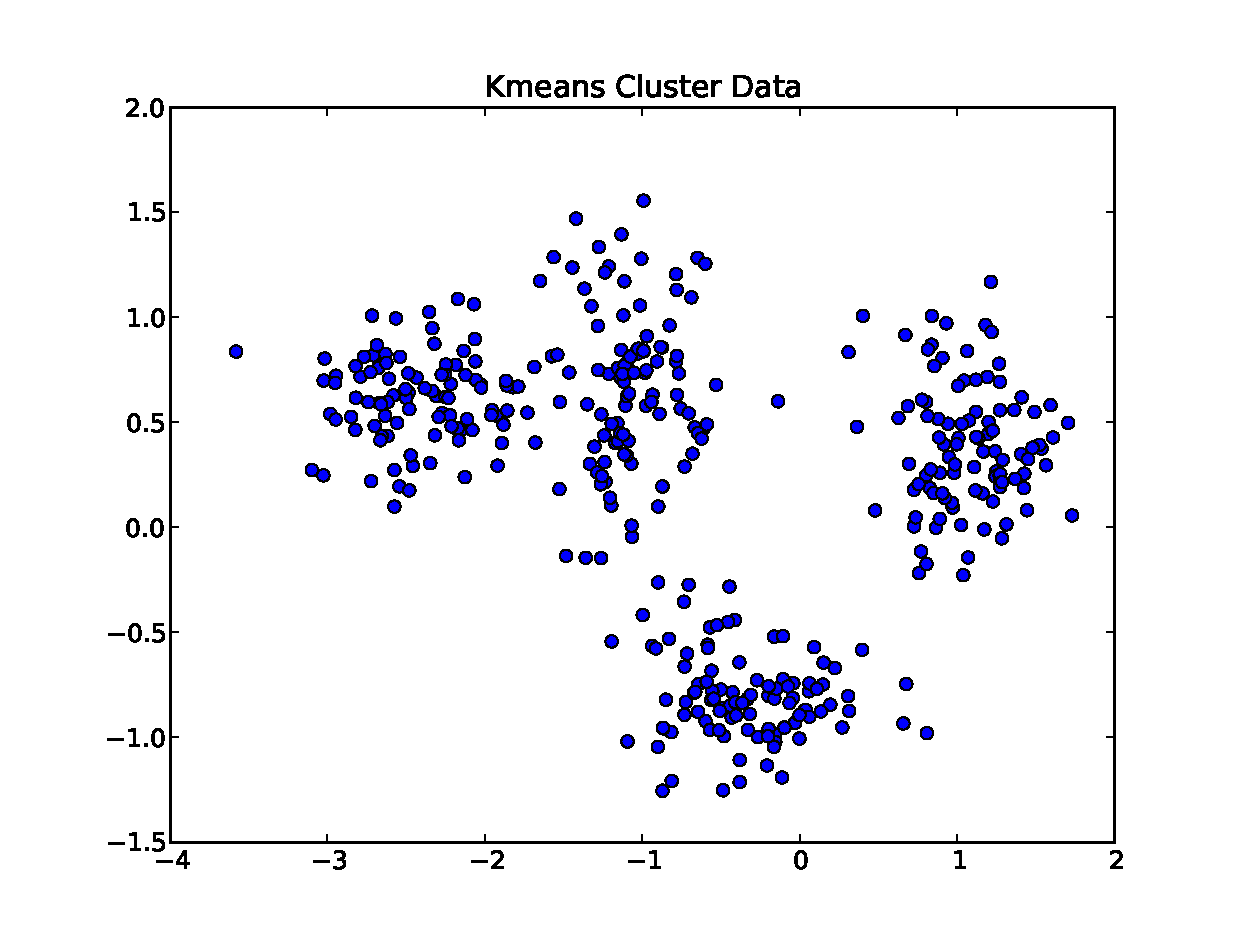
\includegraphics[width=6in]{kmeans_scatter.eps} \\[15mm]
		
		I see 4 clusters. \\[10mm]
		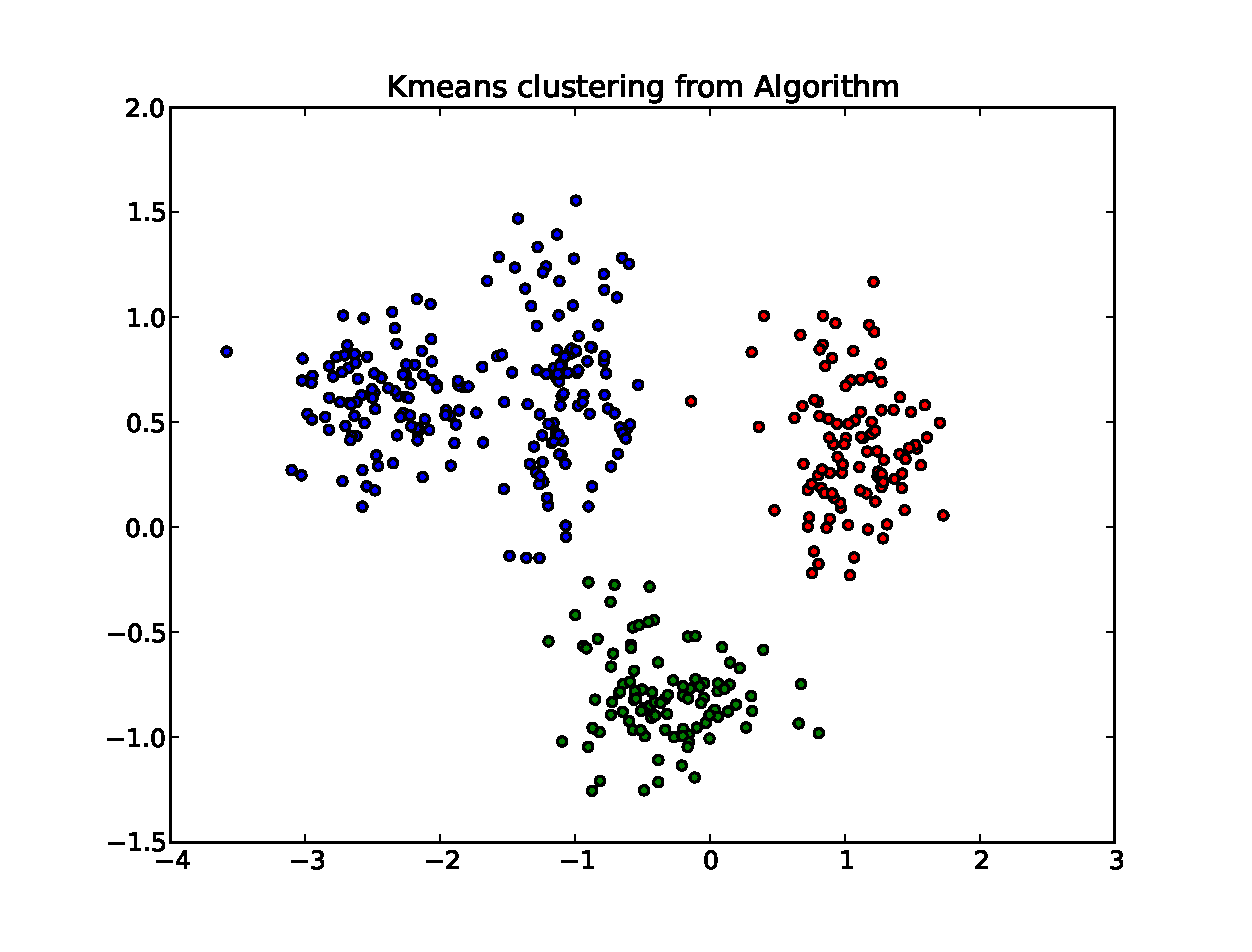
\includegraphics[width=6in]{kmeans_scatter_color.eps} \\[15mm]
		The above graph is the kmeans clustering determined by our algorithm. Each color is associated with a cluster. \\
		\item Now apply your kmeans implementaion to this dat with differnet values of k $(2,3, \ldots, 6$. For each value of k, please run your algorithm 10 times, each time with a different random initialization, record the lowest SSE value achieved in these 10 repeats for each value of k. Plot the recorded SSE values against the changing k value. Does the curve confirm your belief about the k value? Why or why not? \\
		
	\end{enumerate} 
\end{enumerate} 
\end{document} 
